\documentclass[12pt, a4paper]{article}

\usepackage{amssymb}
\usepackage{multicol}
\usepackage{enumerate}
\usepackage[top=5em, bottom=5em, left=5em, right=5em]{geometry}
\usepackage{listings}
\usepackage{tikz}
\usetikzlibrary{positioning}

\setlength\parskip{1em}
\setlength\parindent{0em}

\title{Assignment 11}

\author{Hendrik Werner s4549775}

\begin{document}
\maketitle

\section{} %1
The minimal cut for this graph is $(\{s, A, B, C\}, \{D, t\})$ with a flow of $5$ which is also the maximum flow for the graph.

\section{} %2

\section{} %3

Graph $G$ contains two strongly connected components. The first one ($X$) consists of $A, D, E, G$ and the other one ($Y$) contains $B, C, F, H$. The component graph thus looks like this:

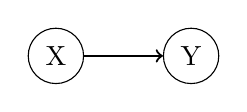
\begin{tikzpicture}[every node/.style={circle, draw, minimum width=2em}]
	\node (A) {X};
	\node [right=of A] (B) {Y};

	\draw[->, thick] (A) -- (B);
\end{tikzpicture}

\section{} %4

Initial state:

\begin{tabular}{|c|c|c|c|c|c|c|c|}
	\hline
	4 & 3 & 6 & 5 & 2 & 2 & 1 & 6\\
	\hline
\end{tabular}

Merging steps:

\begin{enumerate}
	\item \begin{tabular}{|c|c|c|c|c|c|c|c|}
		\hline
		3 & 4 & 5 & 6 & 2 & 2 & 1 & 6\\
		\hline
	\end{tabular}
	\item \begin{tabular}{|c|c|c|c|c|c|c|c|}
		\hline
		3 & 4 & 5 & 6 & 1 & 2 & 2 & 6\\
		\hline
	\end{tabular}
	\item \begin{tabular}{|c|c|c|c|c|c|c|c|}
		\hline
		1 & 2 & 2 & 3 & 4 & 5 & 6 & 6\\
		\hline
	\end{tabular}
\end{enumerate}

\section{} %5

\end{document}
